\graphicspath{{imgs/}}
\documentclass[main.tex]{subfiles}

\begin{document}
\chapter{Results}\label{chap:results}
This chapter presents the result of the training process. The final network performance is evaluated and the network's extracted features are further analyzed.

\section{Training Results}
The model performs after training (see Figure~\ref{fig:validation}) with a sensitivity of $83.39\%$ on the test set.

\begin{figure}[H]
\begin{center}
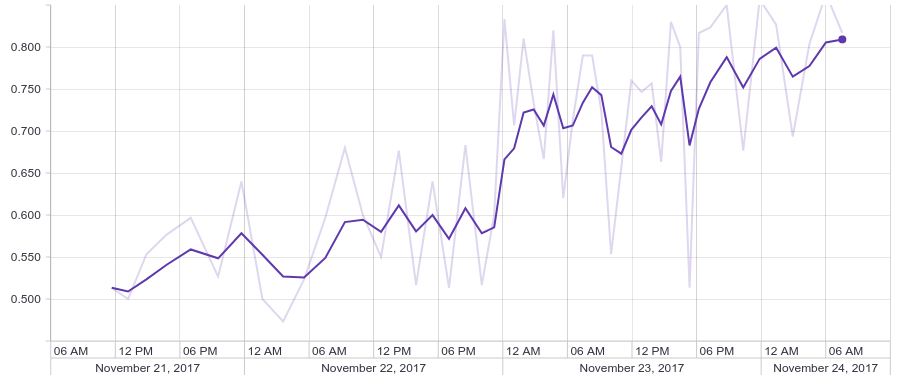
\includegraphics[scale=0.5]{validation_process.png}
\end{center}
\caption{Learning process of the network - the graph shows the development of the accuracy of the network on the validation set. The darker line represents the smoothed values of the lighter line. Since the training is performed on the CPU (GPU cannot be utilized since the network was too big.), it takes several days.}
\label{fig:validation}
\end{figure}

There are other metrics to be accounted for though. The false positive rate in the medical context is crucial since the patients suffer from extreme psychological stress if they are to believe that their cancer screening reveals that they are affected by this severe disease. A false positive error can also lead to increased costs connected to additional screening and testing procedures as well as additional health-related risks for the patients. The false positive rate of the trained model is $0.12$ per sample, which means that roughly every eighth patch is classified wrongly as being a nodule when it is not. Considering the practicability of the approach one would also need to measure the time it takes for the algorithm to analyze a complete CT scan.


\section{Analyzing the Network}
The more interesting part besides the performance measure is the question of how the network solves the task. In this section, the model architecture will be examined, by running the learning process with different parameters. Then the learned features of the final model will be visualized.


\subsection{Model parameters}
Many decisions concerning the architecture have been made that are not cogent. The choice of the activation function, the number of filters and layers as well as the batch size and other values have been either chosen in the beginning or found empirically because they improved the performance of the system. The code structure allows testing easily for the effect of these parameters on the performance. 

\subsubsection{Activation Function}

Figure~\ref{fig:other_act} shows the result of a test run with elu (exponential linear unit) activation function~\ref{eq:elu}, which seemed not to yield very different results.

\begin{equation} \label{eq:elu}
f(x)= \begin{cases}
    x,& \text{if } x\geq 0\\
    \alpha\left(\exp(x) - 1\right), & \text{if } x < 0
    \end{cases}
\end{equation}

\begin{figure}
\begin{center}
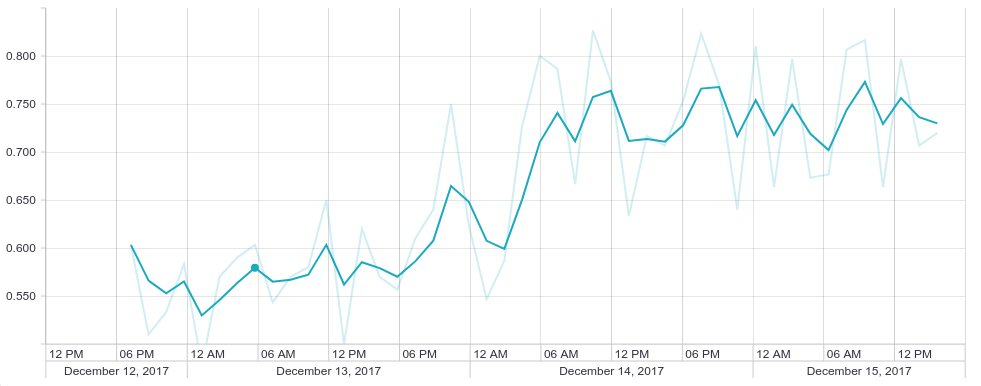
\includegraphics[scale=0.45]{elu_activation.png}
\end{center}
\caption{Using another activation function in the dense layers (elu) shows similar results.}
\label{fig:other_act}
\end{figure}

\subsubsection{Batch Size}

A greater impact on the learning has the batch size. The batch size determines how many samples are fed through the network before applying the gradient optimization step. Without changing the other parameters the learning of the network collapses, as can be seen in Figure~\ref{fig:small_batch}. This can have two reasons. Firstly, the learning rate might be inappropriate for this batch size. A high batch size allows for a higher learning rate since the batch stabilizes the prediction~\footnote{This is only roughly correct. The step size cannot be increased indefinitely since it also depends on the smoothness of the target function (measured by the Lipschitz constant, which is typically not available for the problems that are meant to be solved by the Neural Networks). It is also desirable for the step size to be bigger in the beginning but decaying in the target area to allow for a finer search.}. So it could be that the learning rate is set too high which would explain the high variance in the performance values during training. Because of this, it could also be that the 3 days are simply not enough time to reach an optimum in the problem space.

\begin{figure}[H]
\begin{center}
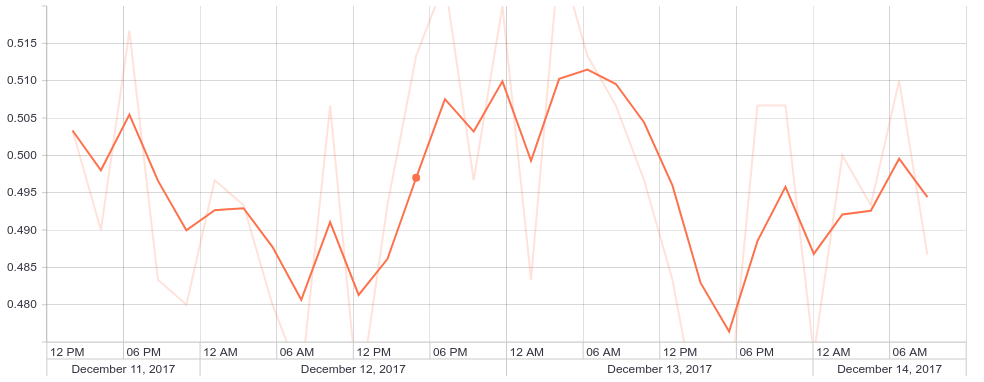
\includegraphics[scale=0.45]{small_batch.png}
\end{center}
\caption{The batch size for this run has been set to 1, decreasing the performance tremendously.}
\label{fig:small_batch}
\end{figure}

\subsubsection{Structural Changes}\label{sss:struct_changes}
 
It is also possible to measure the effect of structural changes to the network. In section~\ref{ss:features} it is revealed that the filters share very similar features, so the effect of reducing the convolutional layers is invested as well as the impact of the dense layer. In Figure~\ref{fig:structure_change} two runs are depicted that show the difference. Reducing the number of convolutional layers had a positive impact on the overall performance of the network while reducing the number of neurons in the flat layer did not yield significant improvements.


\begin{figure}[H]
\begin{center}
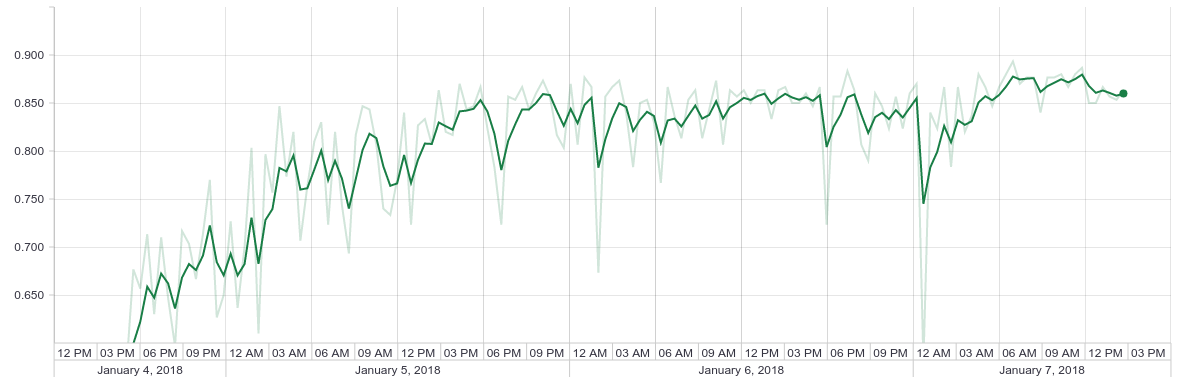
\includegraphics[scale=0.45]{one_conv_perf.png}
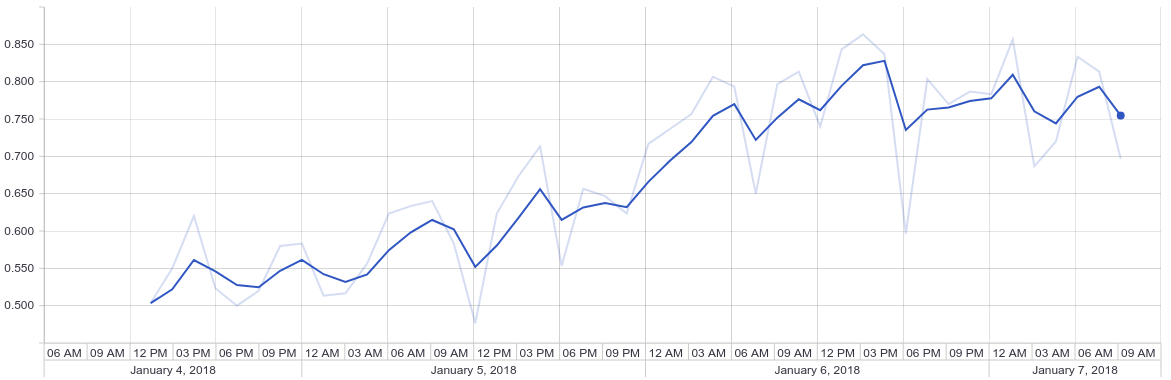
\includegraphics[scale=0.45]{half_flat_performance.png}
\end{center}
\caption{The bottom network was run with only half of the neurons ($32$) in the fully connected layers, while the upper network used only the fist convolutional layer.}
\label{fig:structure_change}
\end{figure}


\subsection{Learned Features}\label{ss:features}
To understand how the network solves the task it makes sense to look at the patterns its layers are sensitive to. The convolutional layers are a suitable target for this kind of inspection since their activation maps can be directly interpreted by visual inspection whereas the activation of the dense layers does not yield such information straight away. Figure~\ref{fig:mean_activation} shows the mean activation of 4 of the kernels in the first layer after passing through 500 nodule patches. Since the nodules are located in the middle of the input the filters respond to that area. The consecutive layers show similar responses (Figure~\ref{fig:mean_activation_l1} and Figure~\ref{fig:mean_activation_l2}). They also show the typical round morphology. This is an indicator that the number of convolutional layers is set too high since they do not learn ever more abstract representations but seem to stick with the features that were found in the first layer. Results like this can be used to further prune and optimize the network as described in Section~\ref{sss:struct_changes}.


\begin{figure}[H]
\begin{center}
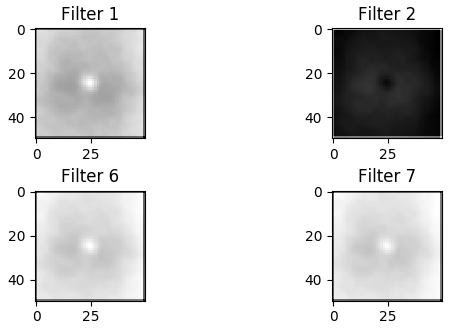
\includegraphics[scale=0.5]{nodule_activation_example.png}
\end{center}
\caption{The mean activation from 500 nodule patches of the validation set. Already in the first layer the receptive field is focusing on the center area, where the nodule resides.}
\label{fig:mean_activation}
\end{figure}

\begin{figure}
\begin{center}
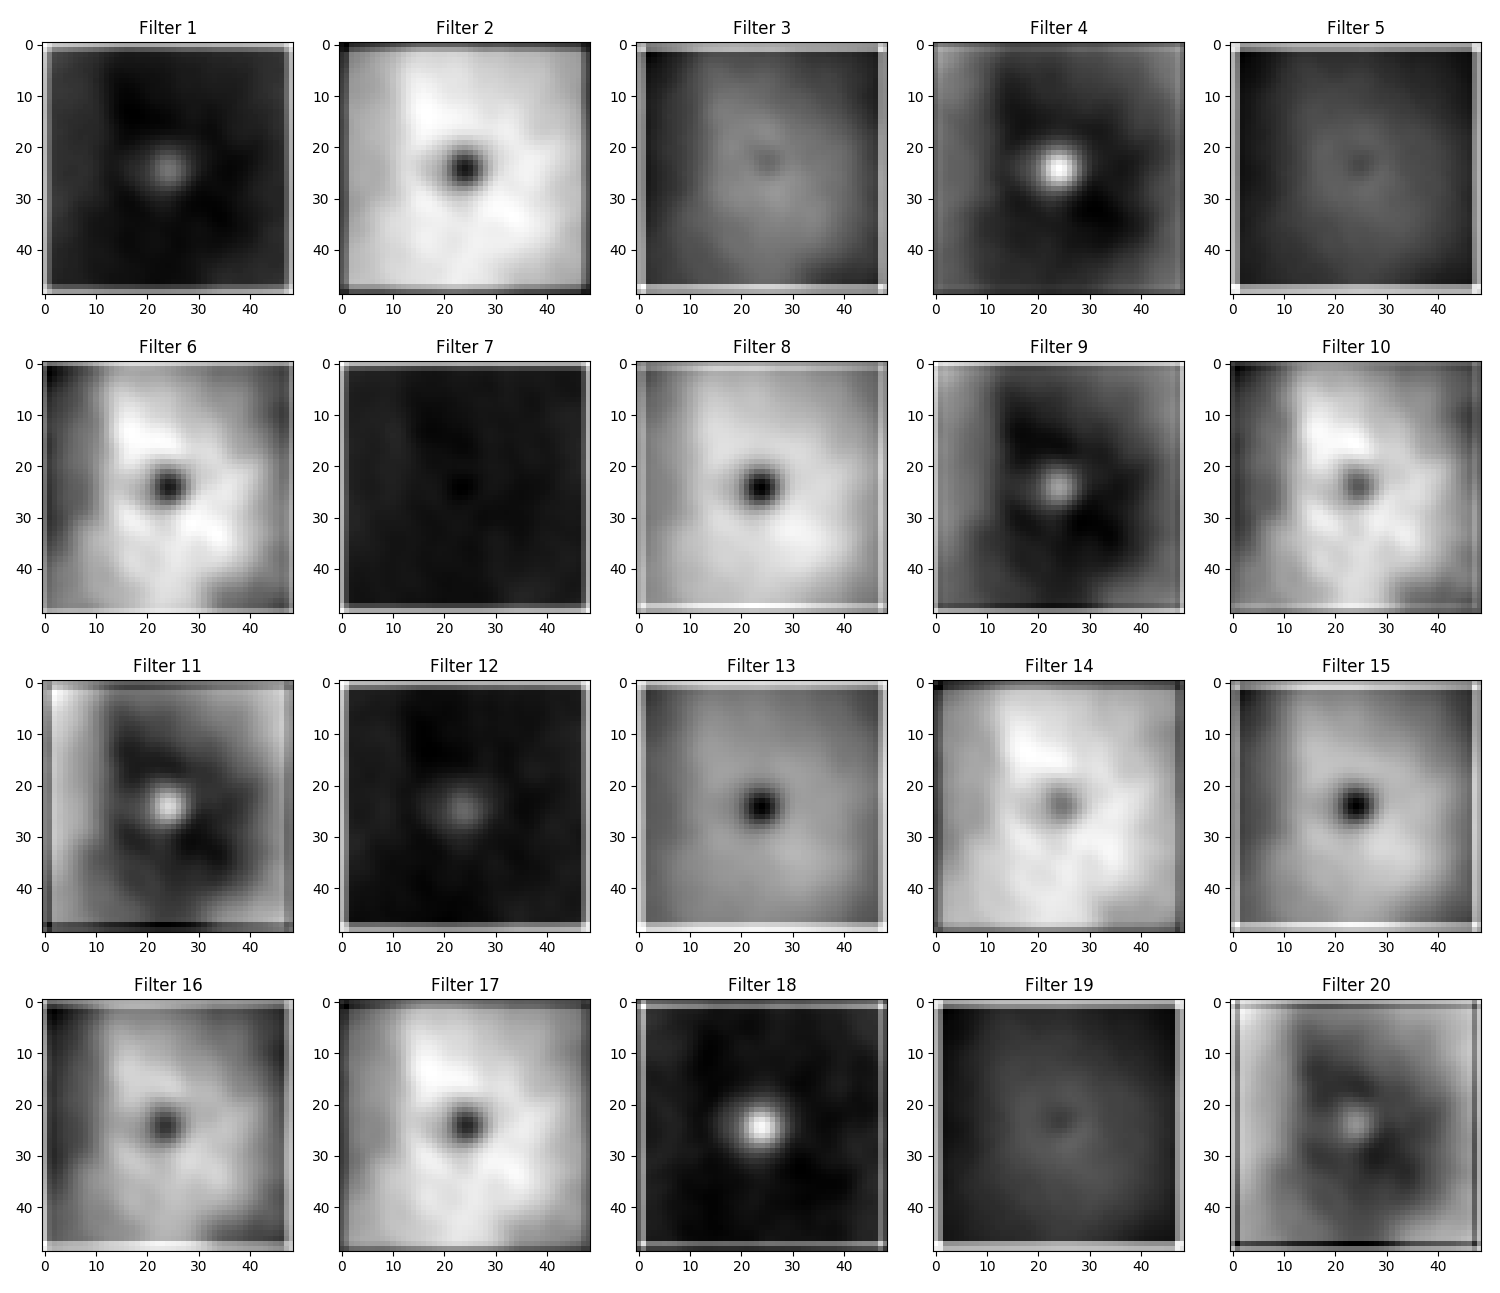
\includegraphics[scale=0.4]{nodule_activation_l1.png}
\end{center}
\caption{The mean activation from 500 nodule patches of the validation set in the second convolutional layer.}
\label{fig:mean_activation_l1}
\end{figure}

\begin{figure}
\begin{center}
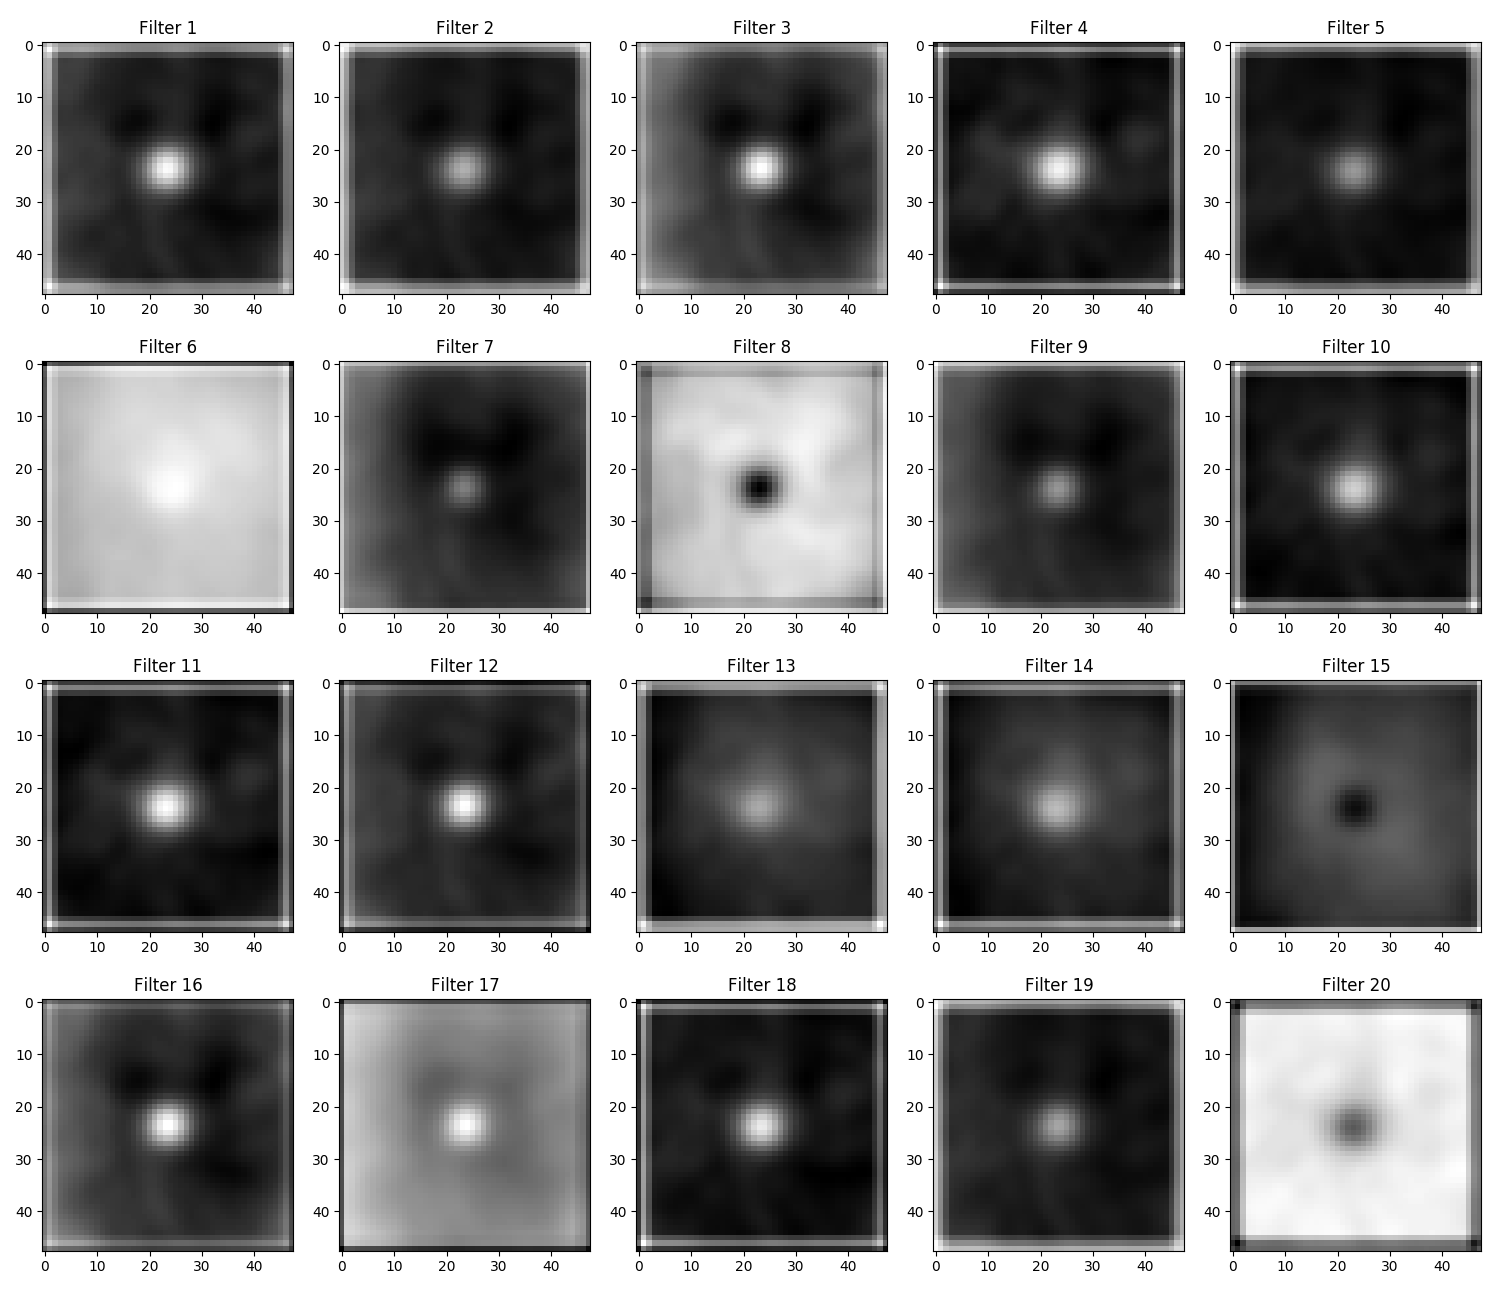
\includegraphics[scale=0.4]{nodule_activation_l2.png}
\end{center}
\caption{The mean activation from 500 nodule patches of the validation set in the third convolutional layer.}
\label{fig:mean_activation_l2}
\end{figure}

\begin{figure}
\begin{center}
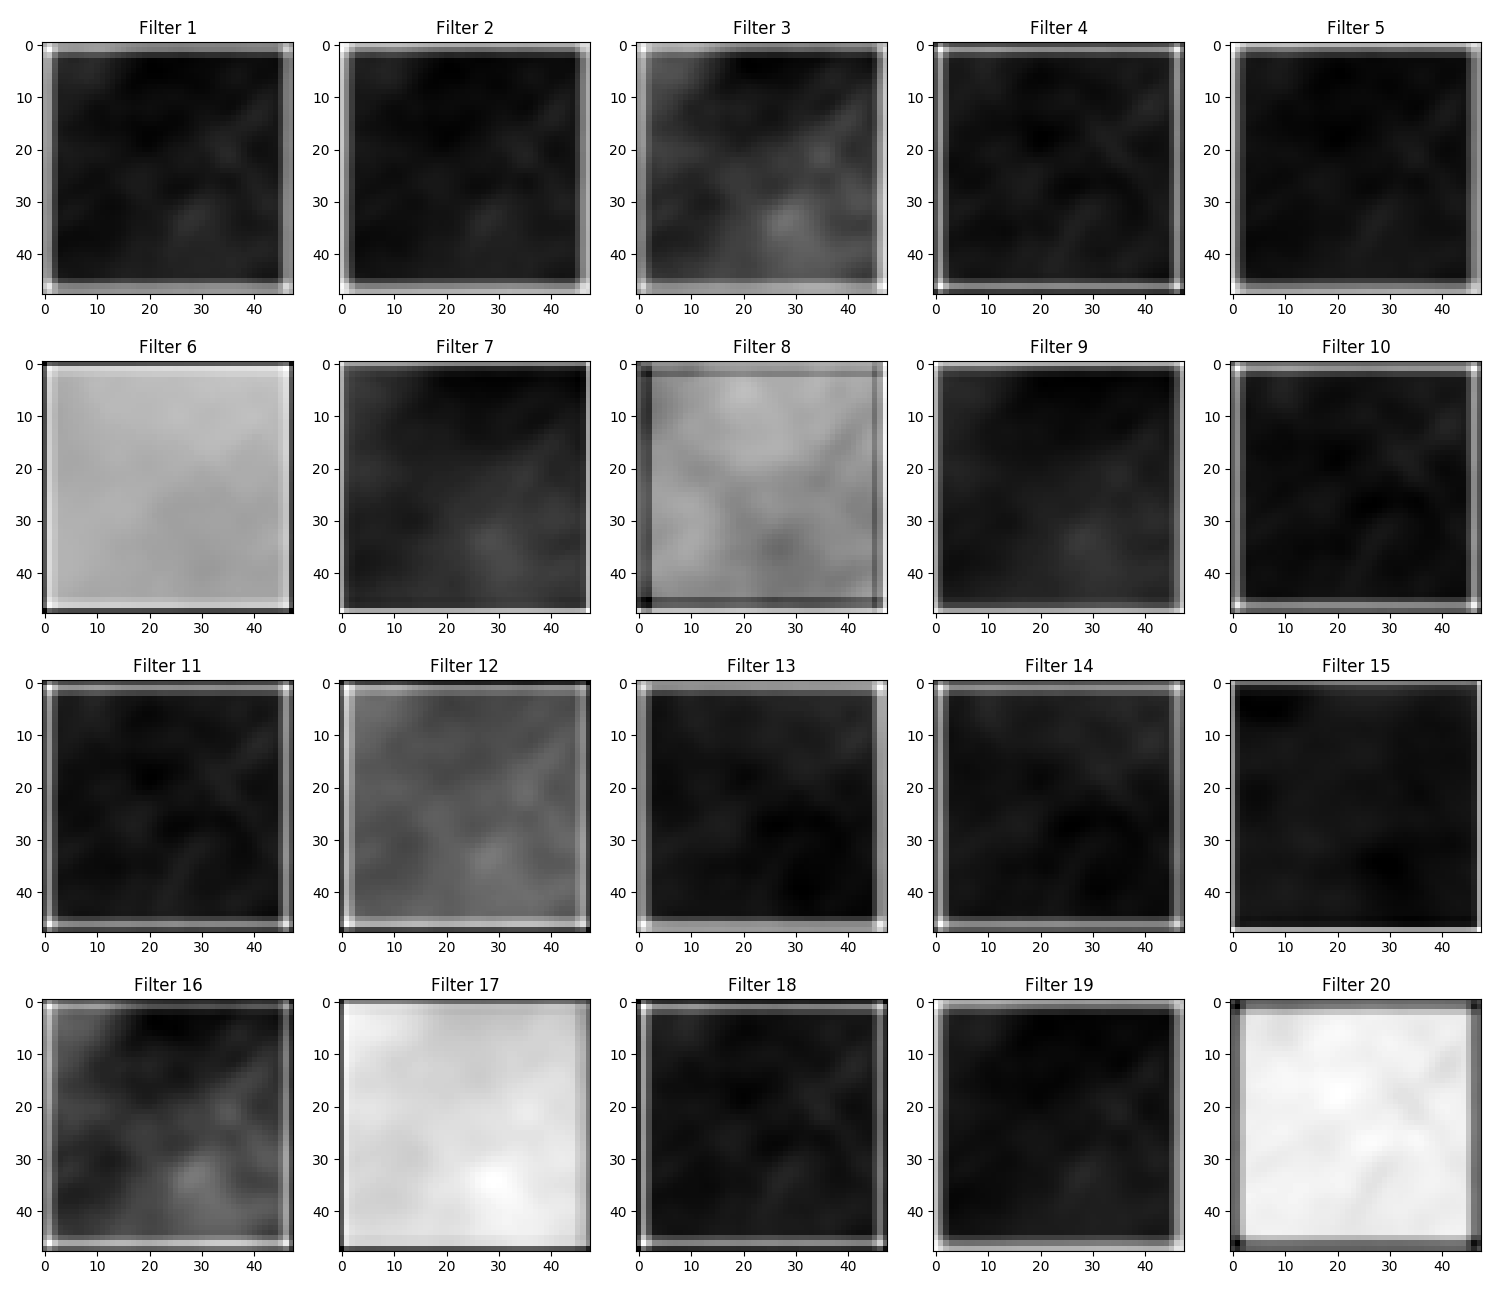
\includegraphics[scale=0.4]{health_activation_l2.png}
\end{center}
\caption{The mean activation from 500 healthy patches of the validation set in the third convolutional layer. Compared to the activations for the nodule patches do those not show a clear pattern.}
\label{fig:mean_activation_l2_health}
\end{figure}


\begin{figure}
\begin{center}
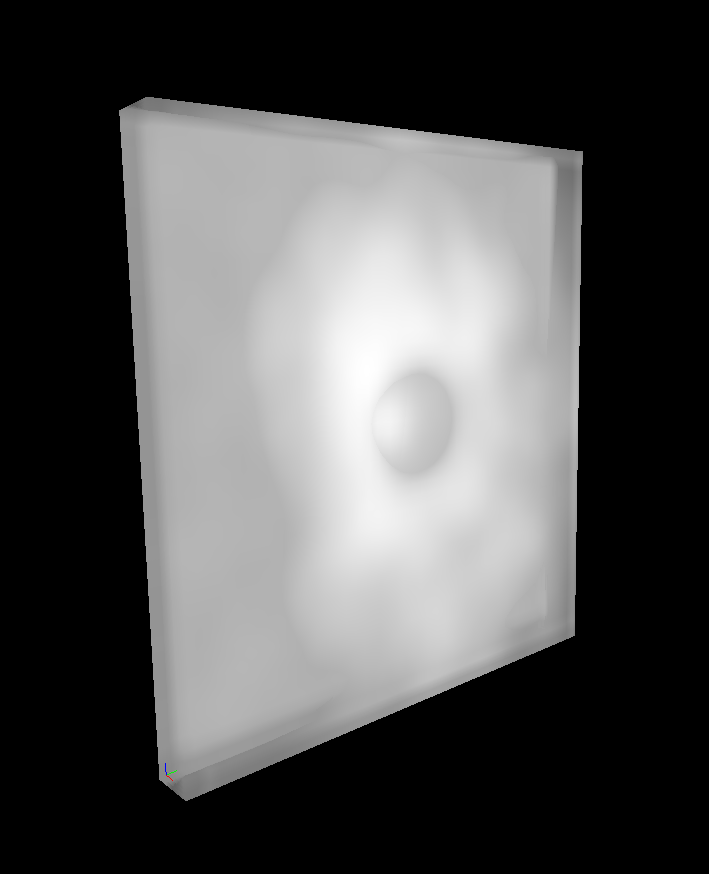
\includegraphics[scale=0.4]{filter9_second_layer.png}
\end{center}
\caption{A visualization of the three dimensional nodule activation of a kernel from the second layer. This visualization was created with the Vispy package~(http://vispy.org/index.html).}
\label{fig:3d_activation}
\end{figure}

\end{document}